\documentclass{article}
\usepackage[utf8]{inputenc}
\usepackage[spanish]{babel}
\usepackage{amsmath}
\usepackage{amssymb}
\usepackage{amsfonts}
\usepackage{hyperref}
\usepackage{textcomp}
\usepackage{graphicx}
\usepackage{pgfplots}
\hypersetup{
    colorlinks=true,
    linkcolor=black,
    citecolor=green,
    filecolor=magenta,      
    urlcolor=cyan,
}

\title{Estadística 1}
\author{Jorge Miguel Alvarado Reyes}
\date{16 Agosto 2023}

\begin{document}

\begin{titlepage}
    \begin{center}
        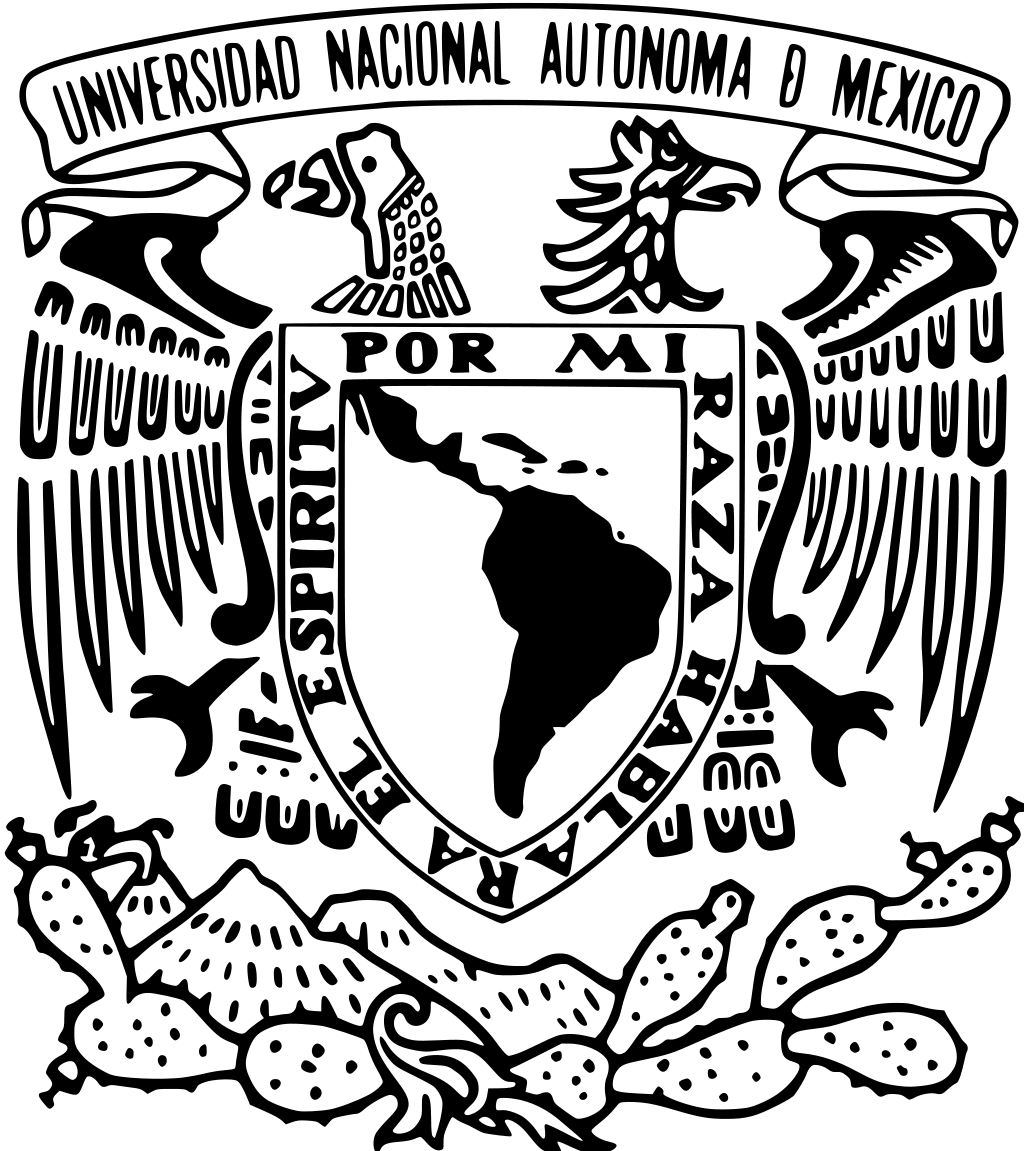
\includegraphics[width=0.2\textwidth]{unam.png}
        \vspace*{.5cm}

        \LARGE
        \textbf{Universidad Nacional Autónoma de México}

        \vspace{0.5cm}
        \LARGE
        Facultad de Estudios Superiores Acatlán

        \vspace{2cm}

        \textbf{Apuntes} \\
        Estadística

        \vfill

        \vspace{1cm}

        \textbf{\large Autor:} \\
        Jorge Miguel Alvarado Reyes \\
        \vspace{.5cm}
        \normalsize \today

    \end{center}
\end{titlepage}
\newpage

\tableofcontents

\newpage

\section{16 de agosto 2023} %Medidas de Tendencia Central

Las medidas de tendencia central son valores de un conjunto de datos que se encuentran en el centro de los datos ordenados.

\subsection{Medidas de Tendencia Central} %media

\subsubsection{Media}

\noindent Existen dos tipos de media: la aritmética y la ponderada.

\noindent La \textbf{media aritmética} se calcula sumando todos los valores y dividiendo por la cantidad de valores:

\[
    \text{Media}(x) = \frac{\sum_{i=1}^{n} x_i}{n} = \frac{1}{n} \cdot \sum_{i=1}^{n}x_i
\]

\textbf{Propiedades}:
\begin{enumerate}
    \item $Media(cx) = c \cdot Media(x)$
    \item $Media(x+c) = Media(x) + c$
\end{enumerate}

\textbf{Ejemplo 4}:

Mostrar que $Media(x+c) = Media(x) + c$.

\textbf{Demostración}:
\[
    \begin{aligned}
        Media(x+c) & = \frac{x_1+c + \ldots + x_n+c}{n}         \\
                   & = \frac{x_1 + \ldots + x_n + n \cdot c}{n} \\
                   & = \frac{x_1 + \ldots + x_n}{n} + c         \\
                   & = Media(x) + c
    \end{aligned}
\]

\textbf{Ejemplo 5}:

Mostrar que $Media(cx) = c \cdot \text{Media}(x)$.

La \textbf{media ponderada} se define como:
\[
    \overline{x} = \frac{\sum_{i=1}^{n} w_i \cdot x_i}{\sum_{i=1}^{n} w_i}
\]

\subsubsection{Mediana}

\noindent La mediana es el valor central que divide a un conjunto de datos ordenados en dos partes iguales. Si $n$ es par, se calcula como:
\[
    Mediana(x) = \frac{x(\frac{n}{2}) + x(\frac{n}{2} + 1)}{2}
\]

% - Estilos -

\subsubsection{Moda}

\noindent Es el valor que mas se repite en un conjunto  de observaciones. \\
\textbf{Ejemplo 6}:

\begin{enumerate}
    \item $[1,2,3,4,5]$ Aqui no existe moda
    \item $[3,4,4,5,5,6]$ Moda = 4.5
    \item $[3,3,4,5,6,6]$ Moda = 3 y 6
    \item $[2,7,7,7,9]$ Moda = 7
\end{enumerate}

\subsection{Media para una serie de frecuencias}

Si $f_1, ... , f_n$ son las frecuencias de la variable $x$. Entonces.
\[
    Mediana(x) = \frac{\sum^{n}_{i=1}f_i \cdot x_i}{\sum^{n}_{i=1}f_i}
\]


\textbf{Ejemplo 7}: \\
Calcula la media para los siguientes valores
\[
    \begin{tabular}{|c|c|}
        \hline
        $x$ & $f_i$ \\
        \hline
        2   & 4     \\
        5   & 1     \\
        6   & 3     \\
        8   & 4     \\
        \hline
    \end{tabular}
\]

\[
    Mediana(x) = \frac{(2\cdot4) + (5\cdot1) + (6\cdot3) + (8\cdot4)}{4+1+3+4} = \frac{8+5+18+32}{12} = \frac{63}{12}
\]

\subsection{Media para datos agrupados}

Sean $f_1, ... , f_n$ las frecuencias de la varible $x$ y $c_1, ... , c_n$ las marcas de clase, entonces: (Marca de clase es un representante)

\[
    Media(x) = \frac{\sum^{n}_{i=1}f_i \cdot c_i}{\sum^{n}_{i=1}f_i}
\]

\textbf{Ejemplo 8}: \\
Calcula la edad promedio para el siguiente conjunto de datos
\[
    \begin{tabular}{|c|c|}
        \hline
        Adulto                    & 25 \\
        \hline
        Adulto de la tercera edad & 10 \\
        \hline
    \end{tabular}
\]

Adulto, edad = [20,65], $c_1 = 43$ \\
Adulto tercera edad, edad = [65,100], $c_1 = 83$\\

25 veces 43 y 10 veces 83

\[
    Mediana(x) = L_{i} t(\frac{\frac{n}{2} - 3 \sum f_i}{f_{mediana}}) \cdot c \\ \\
\]

\noindent $L_i$ = limite inferior de la clase que contiene la mediana\\
$n$ = frecuencia total \\
$\sum f_i$ = suma de las frecuencias menores a la mediana\\
$f_{mediana}$ = Frecuencia de la clase que contiene la mediana\\
$c$ = longitud del intervalo que contiene la mediana \\

\newpage

\section{18 Agosto 2023}

Sitio del curso: https://piazza.com/unam.mx/other/ei20241 \\
codigo de acceso: 150621

\subsection{Breve introduccion a latex}

LaTeX es una herramienta para crear documentos de una gran
calidad tipográfica, en donde los usuarios se ocupan en mayor
medida del contenido del texto en lugar del formato.

\subsubsection{Principales clases de documentos}

\[
    \begin{tabular}{|c|c|}
        \hline
        Clase   & Proposito                                      \\
        \hline
        article & Articulos de revista                           \\
        report  & Textos largos como tesis o reportes            \\
        book    & Libros o documentos con una estructura similar \\
        lette   & cartas                                         \\
        \hline
    \end{tabular}
\]

\subsubsection{Paquetes}

\[
    \begin{tabular}{|c|c|}
        \hline
        Nombre                    & Función                                  \\
        \hline
        amsmath, amssymb, amsfont & Permiten el uso de símbolos matemáticos. \\
        babel                     & Escribir en diversos idiomas.            \\
        inputec                   & Codificacion de entradas.                \\
        \hline
    \end{tabular}
\]

\subsubsection{Estructura de un documento}

\begin{verbatim}
    \documentclass[11pt, a4paper]{report}
    \usepackage[utf8]{inputec}
    \usepackage[spanish]{babel}
    \usepackage{amsmath}
    \usepackage{amssymb}
    \usepackage{amsfont}
    
    \title{Titulo}
    \author{Nombre}
    \date{\today}
    \begin{document}
    \maketitle
    ...
    \end{document}
\end{verbatim}

\subsubsection{LaTex en linea}
Crear cuenta en https://es.overleaf.com \\

New project \textrightarrow Blank project \textrightarrow Escribir nombre del documento
\textrightarrow Create

Menu \textrightarrow spell check spanish

\subsubsection{Partes de un documento}

\begin{verbatim}
    \section*{title}
    \subsection*{title}
    \subsubsection*{title}

    \part*{title}
    \chapter*{title}
\end{verbatim}

\subsubsection{Tamaños de fuente}

\begin{verbatim}
    \huge
    \Huge
    \LARGE
    \Large
    \large
    \normalsize
    \small
    \tiny
\end{verbatim}

\subsubsection{Listas numeradas y viñetas}

\begin{verbatim}
    \begin{itemize}[a]
        \item
        \item 
    \end{itemize}

    \begin{enumerate}
        \item
        \item 
    \end{itemize}
\end{verbatim}

\subsubsection{Alineacion de texto}

\begin{verbatim}
    \begin{center}
        ...
    \end{center}
\end{verbatim}

\subsubsection{Composicion de ecuaciones}

\begin{verbatim}
    $x^2+2x+3=0$
\end{verbatim}

\subsubsection{Alinear expresion con algun elemento}

\begin{verbatim}
    \begin{align*}
        c^2 &= a^2 + b^2 \\
        &= 2^2 + 3^2 \\
        &= 13
    \end{align*}
\end{verbatim}

\subsubsection{Tablas}

\begin{verbatim}
    \begin{table}[h]
        \centering
        \begin{tabular}{c | c  c}
            a & b & c\\   
            a & b & c\\   
            a & b & c\\        
        \end{tabular}
    \end{table}

    \begin{table}[h]
        \centering
        \begin{tabular}{| c c c |}
            \hline
            a & b & c\\   
            \hline
            a & b & c\\  
            \hline 
            a & b & c\\
            \hline       
        \end{tabular}
    \end{table}
    
\end{verbatim}

\subsubsection{Como insertar una imagen}

\begin{verbatim}
    \usepackage{graphicx}
    \includegraphics[width = , height = ]{archivo.jpg,png,etc.}
\end{verbatim}

\newpage

\subsection{Clase}

\textbf{Ejemplo 9}:

Encuentran la mediana para las siguientes observaciones

\begin{table}[h]
    \centering
    \begin{tabular}{| c | c | c |}
        \hline
        Intervalo      & Frecuencia & Frecuencia acumulada \\
        \hline
        (118.5,126.5]  & 3          & 3                    \\
        \hline
        (126.5,135.5]  & 5          & 8                    \\
        \hline
        (135.5,144.5]  & 9          & 17                   \\
        \hline
        (144.5,153.5]  & 12         & 29                   \\
        \hline
        (153.5,162.5]  & 5          & 34                   \\
        \hline
        (162.5,171.5]  & 4          & 38                   \\
        \hline
        (171.5, 180.5] & 2          & 40                   \\
        \hline
    \end{tabular}
\end{table}

\noindent $L_i$ = limite inferior de la clase que contiene la mediana\\
$n$ = frecuencia total \\
$\sum f_i$ = suma de las frecuencias menores a la mediana\\
$f_{mediana}$ = Frecuencia de la clase que contiene la mediana\\
$c$ = longitud del intervalo que contiene la mediana \\

\noindent $L_i$ = 144.5\\
$n$ = 40\\
$\sum f_i$ = 17\\
$f_{mediana}$ = 12 \\
$c$ = 153.5 - 144.5 = 9\\

\begin{align*}
    Mediana(x) & = \frac{x_{20} + x_{21}}{2} = 146.75                         \\
               & = L_i + (\frac{\frac{n}{2} - \sum f_i}{f_{mediana}}) \cdot c \\
\end{align*}

\section{21 Agosto 2023}

\subsection{Medidas de posición (1.6.4)}

\subsubsection{Cuantiles}
\noindent Sean $x_1, \dots , x_n$ observaciones de una variable aleatoria $x$ y $p \in (0,1)$. Un cuantil al $100p\%$ es el numero c que cumple con las siguientes condiciones.

\begin{itemize}
    \centering
    \item $\frac{\#\{x_i|x_i \leq c\}}{n} \geq p$
    \item $\frac{\#\{x_i|x_i \leq c\}}{n} \geq 1 - p$
\end{itemize}

Casos particulares

\begin{itemize}
    \centering
    \item Deciles: si $p = \{0.1, \dots, 0.9\}$
    \item Cuartiles: si $p = \{0.25, 0.50, 0.75\}$
    \item Percentiles: si $p = \{0.01, 0.02, \dots, 0.99\}$
\end{itemize}

\textbf{Ejemplo 10}

Calcula los \underline{deciles} de la variable $x = \{0.1\}$

Supongamos:

Si c=0

\begin{itemize}
    \centering
    \item $\frac{\#\{x_i|x_i \leq 0\}}{n} \geq p$

          $\frac{\#\{0\}}{2} \geq p$

          $\frac{1}{2} \geq p$

          $p = \{$0.1, 0.2, 0.3, 0.4, 0.5$\}$
    \item $\frac{\#\{x_i|x_i \geq 0\}}{n} \geq 1 - p$

          $\frac{\#\{0,1\}}{2} \geq 1 - p$

          $1 \geq 1 - p$

          $p = \{$0.1, 0.2, 0.3, \dots, 0.8, 0.9$\}$
\end{itemize}

Si c=1

\begin{itemize}
    \centering
    \item $\frac{\#\{x_i|x_i \leq 1\}}{n} \geq p$

          $\frac{\#\{0,1\}}{2} \geq p$

          $1 \geq p$

          $p = \{$0.5, 0.6, 0.7, 0.8, 0.9$\}$ ??? para todos no?
    \item $\frac{\#\{x_i|x_i \geq 1\}}{n} \geq 1 - p$

          $\frac{\#\{1\}}{2} \geq p$

          $\frac{1}{2} \geq 1 - p$

          $p = \{$0.5, 0.6, 0.7, 0.8, 0.9$\}$\end{itemize}

\begin{itemize}
    \item q(0.1) = 0
    \item q(0.2) = 0
    \item q(0.3) = 0
    \item q(0.4) = 0
    \item q(0.5) = 0.5
    \item q(0.6) = 1
    \item q(0.7) = 1
    \item q(0.8) = 1
    \item q(0.9) = 1
\end{itemize}

\textbf{Ejemplo 11}

Calcula los cuartiles cd la variable $x=\{0,1,2,3\}$, $n=4$

Si c=0

\begin{itemize}
    \centering
    \item $\frac{\#\{x_i|x_i \leq 0\}}{n} \geq p$

          $\frac{\#\{0\}}{4} \geq p$

          $\frac{1}{4} \geq p$

          $p = \{$0.25$\}$
    \item $\frac{\#\{x_i|x_i \geq 0\}}{n} \geq 1 - p$

          $\frac{\#\{0, 1, 2, 3\}}{4} \geq 1 - p$

          $1 \geq 1 - p$

          $p = \{$0.25, 0.50, 0.75$\}$\end{itemize}

Si c=1

\begin{itemize}
    \centering
    \item $\frac{\#\{x_i|x_i \leq 1\}}{n} \geq p$

          $\frac{\#\{0, 1\}}{4} \geq p$

          $\frac{1}{2} \geq p$

          $p = \{$0.25, 0.5$\}$

    \item $\frac{\#\{x_i|x_i \geq 1\}}{n} \geq 1 - p$

          $\frac{\#\{1,2,3\}}{4} \geq 1 - p$

          $\frac{3}{4} \geq 1 - p$

          $p = \{$0.75$\}$

\end{itemize}

Si c=2

\begin{itemize}
    \centering
    \item $\frac{\#\{x_i|x_i \leq 2\}}{n} \geq p$

          $\frac{\#\{0, 1, 2\}}{4} \geq p$

          $\frac{3}{4} \geq p$

          $p = \{$0.75$\}$

    \item $\frac{\#\{x_i|x_i \geq 2\}}{n} \geq 1 - p$

          $\frac{\#\{2,3\}}{4} \geq 1 - p$

          $\frac{1}{2} \geq 1 - p$

          $p = \{$0.50, 0.75$\}$

\end{itemize}

Si c=3

\begin{itemize}
    \centering
    \item $\frac{\#\{x_i|x_i \leq 3\}}{n} \geq p$

          $\frac{\#\{0, 1, 2, 3\}}{4} \geq p$

          $1 \geq p$

          $p = \{$0.25, 0.5, 0.75$\}$

    \item $\frac{\#\{x_i|x_i \geq 3\}}{n} \geq 1 - p$

          $\frac{\#\{3\}}{4} \geq 1 - p$

          $\frac{1}{4} \geq 1 - p$

          $p = \{$0.75$\}$

\end{itemize}

\begin{itemize}
    \item q(0.25) = 0.5
    \item q(0.50) = 1.5
    \item q(0.75) = 2.5
\end{itemize}

\subsubsection{Varianza}

\noindent Sean $x_1, \dots , x_n$ observaciones de la variable aleatoria x. La varianza de x es
\[
    var(x)=\frac{1}{n} \sum_{i=1}^{n}(x_i-\bar{x})^2=s_x
\]
\[
    \bar{x} = \frac{1}{n} \sum_{i=1}^{n}x_i
\]

Propiedades de la varianza

\begin{center}
    $var(x+c) = var(x)$ \\
    \vspace{.25cm}
    $var(ax) = a^2var(x)$
\end{center}

\newpage

\textbf{Ejemplo 12}

Muestra que $var(ax) = a^2var(x)$

Demostracion:

\begin{align*}
    var(ax) & = \frac{1}{n} \sum_{i=1}^{n}(ax_i - a\bar{x})^2   \\
            & = \frac{1}{n} \sum_{i=1}^{n}(a(x_i - \bar{x}))^2  \\
            & = a^2 \frac{1}{n} \sum_{i=1}^{n}(x_i - \bar{x})^2 \\
            & = a^2 var(x)
\end{align*}

\subsubsection{Desviacion estandar}

\noindent Sean $x_1, \dots, x_n$ observaciones de la variable x.la desviacion estandar de x es

\[
    De(x)=\sqrt{var(x)}
\]

\[
    De(x)=\sqrt{\frac{1}{n} \sum_{i=1}^{n}(x_1-\bar{x})^2}
\]

Propiedades

\begin{center}
    $De(x+c) = De(x)$ \\
    \vspace{.25cm}
    $De(ax) = |a|De(x)$
\end{center}

\subsubsection{Desviacion media}

\noindent Sean $x_1, \dots, x_n$ observaciones de la variable x.la desviacion media de x es

\[
    Dm(x)=\frac{1}{n} \sum_{i=1}^{n}|x_i - \bar{x}|
\]

Propiedades

\begin{center}
    $Dm(x+c) = Dm(x)$ \\
    \vspace{.25cm}
    $Dm(ax) = |a|Dm(x)$
\end{center}

\subsubsection{Rango}

\noindent Sean $x_1, \dots, x_n$ observaciones de la variable x.El rango de x es

\[
    R(x) = x_n-x_1
\]

Propiedades

\begin{center}
    $R(x+c) = R(x)$ \\
    \vspace{.25cm}
    $R(ax) = |a|R(x)$
\end{center}

\textbf{Ejemplo 13} (ejercicio)

Muestra que $var(x+c) = var(x)$

\subsection{Medidas de forma (1.6.5)}

\noindent Sean $x_1, \dots, x_n$ observaciones de la variable x. El k-esimo momento de x es

\[
    m'_k(x) = \frac{1}{n} \sum_{i=1}^{n}x_i^k
\]

Mientras que el k-esimo momento central de x es

\[
    m_k(x) = \frac{1}{n} \sum_{i=1}^{n}(x_i - \bar{x})^k
\]

\subsubsection{Asimetria}

\noindent El coeficiente de asimetria mide la asimetria de los datos respecto a la media.

\noindent Sean $x_1, \dots, x_n$ observaciones de la variable x. El coeficiente de asimetria de x es

\[
    sk(x) = \frac{1}{s^3}[\frac{1}{n} \sum_{i=1}^{n}(x_i - \bar{x})^3]
\]

Donde s es la desviacion estandar de x.

\newpage

\section{23 agosto 2023}

\subsection{Medidas de forma (1.6.5) (continuacion)}

\subsubsection{Coeficiente de asimetria}

\[
    sk(x) = \frac{1}{s^3}[\frac{1}{n} \sum_{i=1}^{n}(x_i - \bar{x})^3]
\]

Donde s es la desviacion estandar de x.

\begin{align*}
    sk(x) & = \frac{1}{s^3}[m_3]              \\
          & = \frac{m_3}{(m_2)^{\frac{3}{2}}}
\end{align*}

Donde:

\[
    s = (\frac{1}{n} \sum_{i=1}^{n}(x_i-\bar{x})^2)^{\frac{1}{2}}
\]

\begin{figure}[htbp]
    \centering
    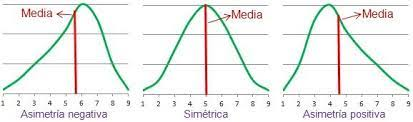
\includegraphics[width=0.5\textwidth]{imagen1.jpeg}
    \caption{negativa = $sk(x) < 0$, Simetrica = $sk(x) = 0$, positiva = $sk(x) > 0$}
    \label{fig:imagen1}
\end{figure}

\textbf{Ejemplo 14}

\noindent Muestra que el coeficiente de asimetria es adimensional e invariante a cambios de escala y origen.

\begin{center}
    $sk(ax+c) = sk(x)$
\end{center}

Demostracion:

\noindent Debido a que $m_3$ y $(m_2)^{\frac{3}{2}}$ tienen la misma unidad de medida, sk(x) es adimensional.

\begin{align*}
    sk(ax+c)    & = \frac{1}{(s(ax+c))^3}[\frac{1}{n} \sum_{i=1}^{n}((ax+c) - (a\bar{x}+c))^3] \\
    Media(ax+c) & = aMedia(x) + c                                                              \\
    s(ax+c)     & = |a|s(x)                                                                    \\
                & = \frac{1}{[|a|s(x)]^3}[\frac{a^3}{n}\sum_{i=1}^{n}(x_i-\bar{x})^3]          \\
                & = \frac{a^3}{|a|^3} \frac{1}{s^3}[\frac{1}{n}\sum_{i=1}^{n}(X_i-\bar{x})^3]  \\
                & = \frac{a^3}{|a|^3} sk(x)
\end{align*}

\subsubsection{Curtosis}

\noindent Sean $x_1, \dots, x_n$ observaciones de la variable x. La curtosis de x se define como.

\begin{align*}
    k(x) & = \frac{1}{s^4}[\frac{1}{n}\sum_{i=1}^{n}(x_i - \bar{x})^4] \\
         & = \frac{m_4}{(m_2)^2}
\end{align*}

\subsubsection{Coeficiente de Fisher}

\[
    k_3(x)=k(x)-3
\]

\begin{figure}[htbp]
    \centering
    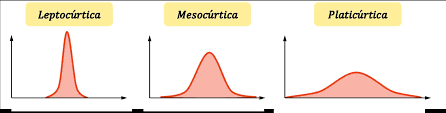
\includegraphics[width=0.7\textwidth]{imagen2.png}
    \caption{}
    \label{fig:imagen2}
\end{figure}

\newpage

\subsection{Medidas de asociacion (1.6.6)}

\begin{figure}[htbp]
    \centering
    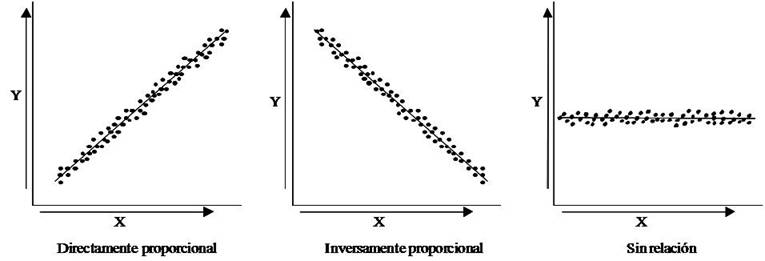
\includegraphics[width=0.7\textwidth]{imagen3.jpg}
    \label{fig:imagen3}
\end{figure}

\subsubsection{Covarianza}

\noindent Sean $(x_1, y_1) \dots, (x_n, y_n)$ observaciones de las variables (x,y). La covarianza entre las variables (x,y) se define como

\[
    s_{xy} = \frac{1}{n}\sum_{i=1}^{n}(x_i-\bar{x})(y_i - \bar{y})
\]

\textbf{Ejemplo 15}

Muestra que

\[
    s_{xy} = \frac{1}{n}[\sum_{i=1}^{n}x_iy_i-n\bar{x}\bar{y}]
\]

\begin{align*}
    s_{xy} & = \frac{1}{n}\sum_{i=1}^{n}(x_i-\bar{x})(y_i - \bar{y})                                                                   \\
           & = \frac{1}{n}\sum_{i=1}^{n}(x_iy_i - x_i\bar{y} - y_i\bar{x} + \bar{x}\bar{y})                                            \\
           & = \frac{1}{n} [\sum_{i=1}^{n}x_iy_i - \sum_{i=1}^{n}x_i\bar{y} - \sum_{i=1}^{n}y_i\bar{x} + \sum_{i=1}^{n}\bar{x}\bar{y}] \\
           & = \frac{1}{n} [\sum_{i=1}^{n}x_iy_i - n\bar{x}\bar{y} - n\bar{x}\bar{y} + n\bar{x}\bar{y}]                                \\
           & = \frac{1}{n}[\sum_{i=1}^{n}x_iy_i - n\bar{x}\bar{y}]
\end{align*}

\begin{center}
    Nota:\\
    $n\bar{x}\bar{y} = n \frac{\sum x_i}{n} \bar{y} = \sum x_i \bar{y}$
\end{center}

\newpage

\subsubsection{Coeficiente de correlacion de Pearson}

\noindent Sean $(x_1, y_1) \dots, (x_n, y_n)$ observaciones de las variables (x,y). El coeficiente de correlacion de Pearson entre las variables (x,y) se define como

\[
    r_xy = \frac{s_{xy}}{s_xs_y}
\]
Donde $s_x$ es la desviacion estandar de x y $s_y$ es la desviacion estandar de y \\

Alguna consideraciones del coeficiente de correlacion son las siguientes:

\begin{center}
    $r_{xy} \in [-1,1]$ \\
    si $x \bot y, r_{xy} = 0$ \\
    si $r_{xy} < 0$, relacion inversa entre las variables
\end{center}

\subsection{Presentacion grafica y tabular de los datos (1.6.7)}

\textbf{Ejemplo 16}

Supongamos que se tiene una variable cualitativa ordinal con valores ordenados de menor a mayor, A,B,C,D,E,F con las siguientes frecuencias,

\begin{table}[h]
    \centering
    \begin{tabular}{|c c c c c|}
        \hline
        Valor & F absoluta & F absoluta acumulada & F relativa & F relativa acumulada \\
        \hline
        A     & 2          & 2                    & 2/28       & 2/28                 \\
        B     & 8          & 10                   & 8/28       & 10/28                \\
        C     & 6          & 16                   & 6/28       & 16/28                \\
        D     & 4          & 20                   & 4/28       & 20/28                \\
        E     & 3          & 23                   & 3/28       & 23/28                \\
        F     & 5          & 28                   & 5/28       & 28/28                \\
        \hline
    \end{tabular}
\end{table}

\newpage

\section{25 agosto 2023}

\subsection{Graficas de barras}

\noindent A cada clase de una variable se le asocia una barra de la altura la frecuencia de las observaciones. Se utiliza para cualquier tipo de variables.

\begin{figure}[htbp]
    \centering
    
\includegraphics[width=0.5\textwidth]{imagen4.png}
    \label{fig:imagen4}
\end{figure}

\subsection{Histograma}

Es una grafica donde los valores de la variable tiene un orden

\begin{figure}[htbp]
    \centering
    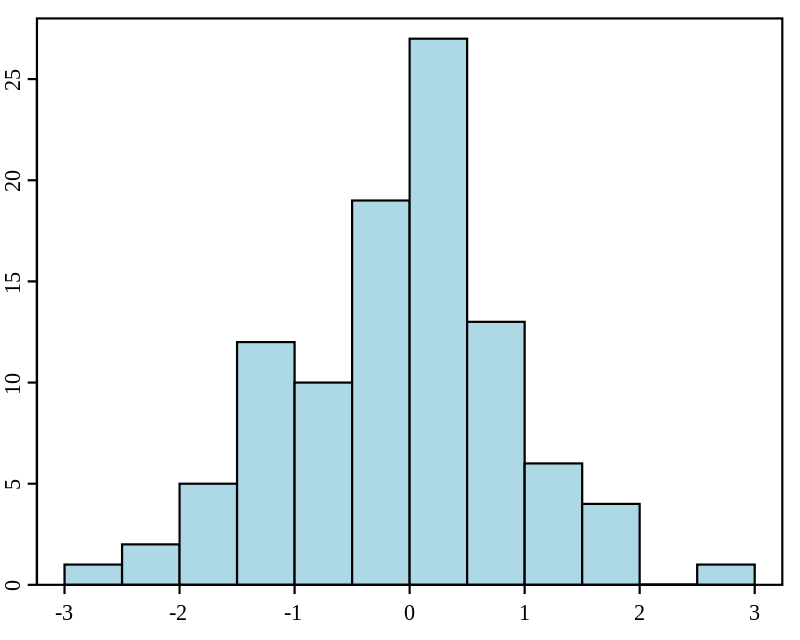
\includegraphics[width=0.5\textwidth]{imagen5.png}
    \label{fig:imagen5}
\end{figure}

\newpage

\subsection{Gráficos de dispersión}

Muestra la relacion entre dos variables

\begin{figure}[htbp]
    \centering
    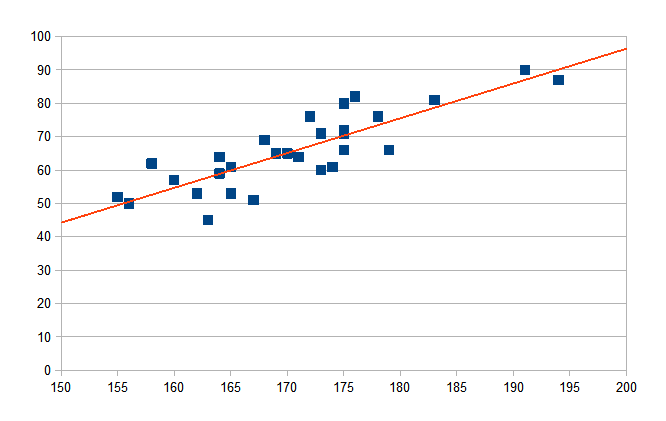
\includegraphics[width=0.5\textwidth]{imagen6.png}
    \label{fig:imagen6}
\end{figure}

\subsection{Gráfica de burbujas}

Muestra la relación para tres variables

\begin{figure}[htbp]
    \centering
    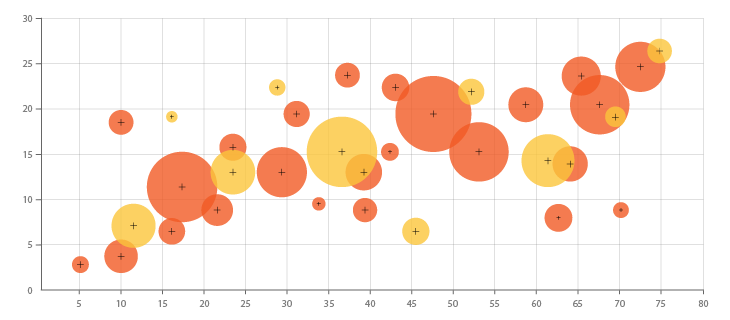
\includegraphics[width=0.6\textwidth]{imagen7.png}
    \label{fig:imagen7}
\end{figure}

\subsection{Serie temporal}

Por medio de una linea se recorren diferentes valores o frecuencias a lo largo del tiempo.

\begin{figure}[htbp]
    \centering
    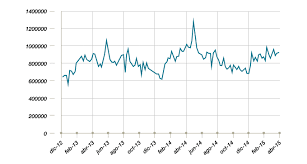
\includegraphics[width=0.6\textwidth]{imagen8.png}
    \label{fig:imagen8}
\end{figure}

\subsection{Introducción a R}

\noindent R es un programa útil para el análisis y visualización de datos. Es abierto y gratuito.

\noindent Es un lenguaje interpretado y tipado.

\noindent Fue creado por Ross lhaka y Robert Gentle-man.

Instalación.

\noindent Descargar R: https://cran.r-project.org/ \\
Descargar R studio: https://posit.co/download/rstudio-desktop/

\subsection{Reglas de sintaxis}

\begin{itemize}
    \item R distingue entre mayúsculas y minúsculas
    \item Los nombres de las variables pueden contener letras, números y puntos. Sin embargo, deben comenzar con una letra y no pueden contener espacion.
          Ejemplo: \\
          Uso correcto \\
          $monto\_total <- 1200$ \\
          $monto\_mensual <- 200$ \\
          Uso incorrecto \\
          $montoTotal <- 1200$ \\
          $MontoMensual <- 200$

    \item Usar espacios alrededor de todos los operadores binarios $(=, +, -, <-, etc)$ y un espacio despúes de una coma.

    \item Ayuda, se puede usar el comando help(mean) o ?mean
    \item Tipos de datos, enteros, númericos y complejos. \\
          Ejemplo: \\
          $entero <- 1L$ \\
          $numerico <- 1$ \\
          $complejo <- 3+4i$ \\
          print(entero, str(entero))
    \item Cadena de texto \\
          Ejemplo: \\
          $mensaje <- "Hola mundo"$ \\
          print(mensaje, str(mensaje))
    \item Factores \\
          Ejemplo: \\
          $colores <- factor(levels = c("azul", "verde"))$ \\
          print(colores)
\end{itemize}

\section{28 agosto 2023}

\subsection{Diagrama de caja y brazos}

\begin{figure}[htbp]
    \centering
    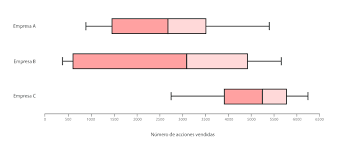
\includegraphics[width=0.6\textwidth]{imagen9.png}
    \label{fig:imagen9}
\end{figure}

\subsection{Continuación de R}

\subsubsection{Operadores aritméticos}

\begin{itemize}
    \item Suma (+)
    \item revista (-)
    \item Multiplicación (*)
    \item División (/)
    \item División entera (\% / \% )
    \item Módulo (\% \%)
\end{itemize}

\subsubsection{Operadores de asignacion}

\begin{itemize}
    \item $valor_1 <- 5$
    \item $valor_2 = 6$
    \item $7 -> valor_3$
\end{itemize}

\subsubsection{Operadores de comparacion e identidad}

\begin{itemize}
    \item Menor
    \item Mayor
    \item Menor o igual
    \item Mayor o igual
    \item Igual
    \item Distinto
\end{itemize}

\subsubsection{Funciones para cadenas de texto}

\begin{itemize}
    \item paste() Concatena varias cadenas en una sola cadena
    \item rep() Repite un objeto n cantidad de veces
    \item grepl() Busca un patron en una cadena de texto y devuelve un vector logico
\end{itemize}

\subsubsection{Listas}

\begin{itemize}
    \item lista <- list(1,"Manzana")
\end{itemize}

\subsubsection{Matrices}

\begin{itemize}
    \item $matriz_1 <- matrix(1:10, nrow=2, ncol=5)$
\end{itemize}

\subsubsection{Convertir tipo de datos}

\begin{itemize}
    \item as.integer
    \item as.numeric
    \item as.complex
    \item as.factor
    \item as.logical
\end{itemize}

\subsection{Funciones con dataFrames}

\begin{itemize}
    \item str()
    \item head()
    \item tail()
    \item summary()
\end{itemize}

\newpage

\section{30 Agosto 2023}

\subsection{Funciones}

\begin{verbatim}
    nombre_funcion <- function(argumentos){
        operaciones
        return(resultado)
    }
\end{verbatim}

\subsection{Unidad 2}

Métodos para la obtención de funciones de variables aleatorias

\vspace{.2cm}

\textbf{Definición}

\vspace{.2cm}

\noindent Consideremos un fenómeno aleatorio junto con un espacio de probabilidad ($\Omega, F, P$). Una variable aleatoria es una transformación $X$ del espacio de resultados $\Omega$ al conjunto de los reales, tal que:

\[
    \{w \in \Omega : X(w) \leq x\} \in F
\]

\vspace{.2cm}

\textbf{Definición}

\vspace{.2cm}

\noindent Una variable aleatoria es discreta cuando el conjunto de valores que toma es un conjunto discreto

\vspace{.2cm}

\textbf{Definición}

\vspace{.2cm}

\noindent Una variable aleatoria en continua cuando el conjunto de valores que toma está en un intervalo $(a,b) \in \mathbb{R}$

\vspace{.2cm}

\textbf{Definición}

\vspace{.2cm}

\noindent Sea $X$ una variable aleatoria discreta con valores $x_0, x_1, \dots$ y probabilidades respectivas $\mathbb{P}(X=x_0), \mathbb{P}(X=x_1), \dots$ la función masa de probabilidad de x denotada por $f(x): \mathbb{R} \rightarrow [0, \infty)$ se define como sigue:

\[
    f(x) = \begin{cases}
        \mathbb{P}(X=x), & \text{si } x = x_1, x_2, \dots, \\
        0,               & \text{c.o.c }.
    \end{cases}
\]

Y cumple con las siguentes Propiedades

\begin{center}
    a) $f(x) \geq 0 \forall x \in \mathbb{R}$ \\
    b) $\sum_{x \in X} f(x) = 1$
\end{center}

\vspace{.2cm}

\textbf{Definición}

\vspace{.2cm}

Sea $X$ una variable aleatoria discreta y $f(x)$ la función masa de probabilidad de $X$, la función de distribución de $X$, denotada por $F(x) \rightarrow [0,1]$ se define como:

\[
    F(x) = \mathbb{P}(X \leq x) = \sum_{x_i\leq x}(f(x_i))
\]

\vspace{.2cm}

\textbf{Definición}

\vspace{.2cm}

Sea $X$ una variable aleatoria continua, decimos que la función integrable $f(x): \mathbb{R} \rightarrow [0, \infty)$ es la función de densidad de $X$ si para cualquier intervalo $(a,b) \in \mathbb{R}$ se cumple que:

\[
    \mathbb{P}(X \in (a,b)) = \int_{a}^{b} f(x) \,dx
\]

y cumple:

\begin{center}
    a)$f(x) \geq 0$ \\
    b)$\int_{-\infty}^{\infty}f(x) = 1$
\end{center}

\vspace{.2cm}

\textbf{Definición}

\vspace{.2cm}

Sea $X$ una variable aleatoria continua y $f(t)$ la función de densidad de $x$, la función de distribución de $X$, denotada por $F(x) = \mathbb{R} \rightarrow [0,1]$, se define como

\[
    F(x) = \mathbb{P}(X \leq x) = \int_{-\infty}^{x}f(t) dt
\]

\vspace{.2cm}

\textbf{Definición}

\vspace{.2cm}

La variable aleatoria $X$ se llama continua si su correspondiente función de distribución es continua y creciente

\vspace{.2cm}

\textbf{Definición}

\vspace{.2cm}

La variable aleatoria $X$ se llama discrtea si su correspondiente función de distribución es constante por pedazos

\vspace{.2cm}

\textbf{Ejemplo}

\vspace{.2cm}

Para cada uno de los siguientes incisos, identifica si la gráfica de la función de distribución corresponde a una variable aleatoria discreta o continua.

\begin{figure}[htbp]
    \centering
    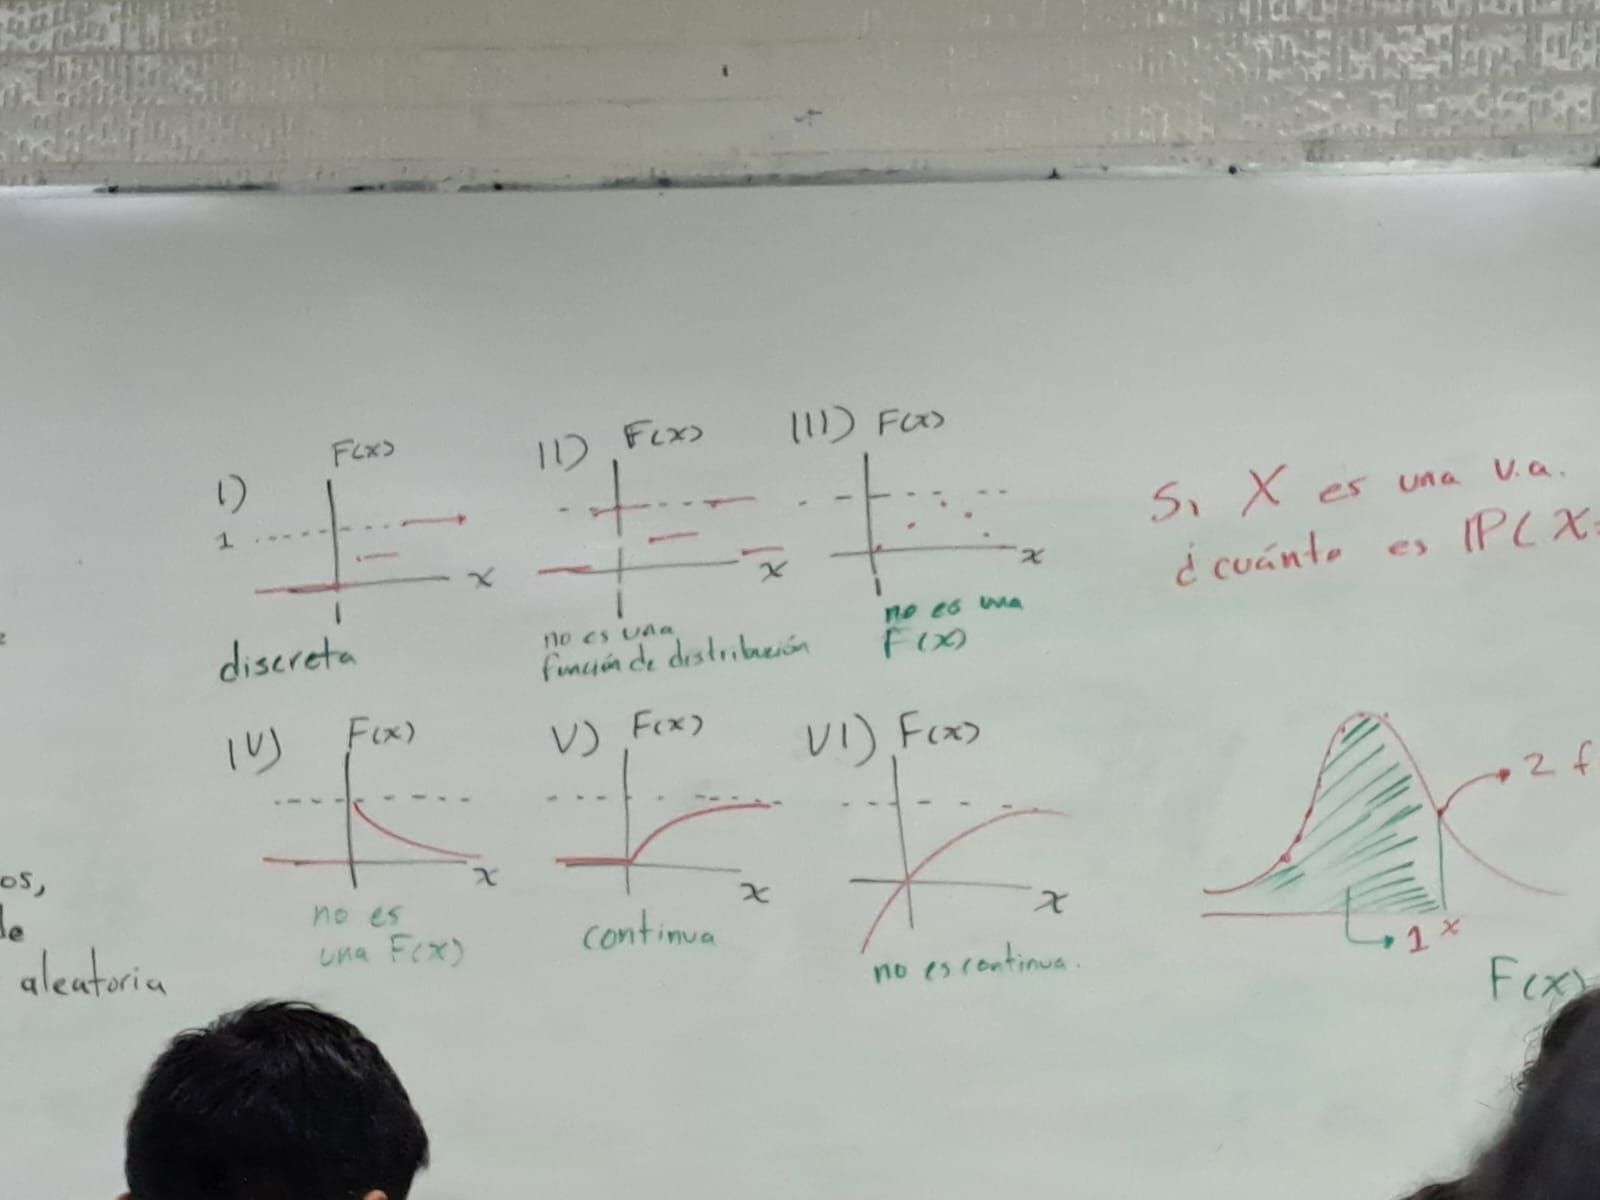
\includegraphics[width=1\textwidth]{Imagen10.jpeg}
    \label{fig:imagen10}
\end{figure}

\newpage

\section{1 Septiembre 2023}

\subsection{Métodos de las funciones de distribución}

\noindent Sea $X$ una variable aleatoria con función de densidad $f(x)$ y $\varphi$ una función de $X$, entonces la variable aleatoria $Y = \varphi(x)$ con funciónde distribución $F_y(y)=\mathbb{P}(Y \leq y)$, $f(y)$ se puede calcular al integrar la región para la cual $Y \leq y$. Ademas, la función de densidad de la variable y se puede calcular al derivar $F_y(y)$\\

\textbf{Ejemplo 2}

Encuentra la función de densidad de la variable $Y$, si $Y=3X-1$ donde.

\[
    f(x) = \begin{cases}
        2x & \text{si } 0 \leq x \leq 1 \\
        0, & \text{c.o.c }.
    \end{cases}
\]

\begin{align*}
    F_y(y) & = \mathbb{P}(Y \leq y)                        \\
           & = \mathbb{P}(3x-1 \leq y)                     \\
           & = \mathbb{P}(3x \leq y + 1)                   \\
           & = \mathbb{P}\left(x \leq \frac{y+1}{3}\right) \\
           & = \int_{0}^{\frac{y+1}{3}} f(x) \, dx
\end{align*}

\begin{itemize}
    \item Si $y=-1$, $\frac{y+1}{3} = 0$
    \item Si $y < -1$ entonces $F_y(y)=0$
    \item Si $y=2$ entonces $F_y(y)=1$
\end{itemize}

\begin{align*}
    F_y(y) & = \int_{0}^{\frac{y+1}{3}} 2x \, dx \\
           & = \frac{(y+1)^2}{9}                 \\
\end{align*}

\[
    F_y(y) = \begin{cases}
        0                  & \text{si } y < -1 \\
        \frac{(y+1)^2}{9}, & -1 \leq y \leq 2  \\
        1                  & \text{si }  y > 2
    \end{cases}
\]

Si derivamos $\frac{d(F_y(y))}{dy}$

\[
    f_y(y) = \begin{cases}
        \frac{2}{9} (y+1)^2 & \text{si } -1 \leq y \leq 2 \\
        0                   & \text{c.o.c}
    \end{cases}
\]

\textbf{Ejemplo 3}

La función de densidad conjunta de $X_1$ y $X_2$ está dada por

\[
    f(x_1, x_2) = \begin{cases}
        3x_1 & \text{si } -0 \leq x_2 \leq x_1 \leq 1 \\
        0    & \text{c.o.c}
    \end{cases}
\]

Encuentra la función de densidad $Y=x_1 - X_2$

\begin{align*}
    F_y(y) & = \mathbb{P}(Y \leq y)                                       \\
           & = \mathbb{P}(X_1 - X_2 \leq y)                               \\
           & = 1 - \mathbb{P}(X_1 - X_2 \leq y)                           \\
           & = 1 - \int_{y}^{1} \int_{0}^{X_1-y} f(x_1, x_2) \, dx_2 dx_1 \\
           & = 1 - \int_{y}^{1} \int_{0}^{X_1-y} 3x_1 \, dx_2 dx_1        \\
           & = 1 - \int_{y}^{1} [3x_1x_2 |_{0}^{x_1-y}] dx_1              \\
           & = 1 - \int_{y}^{1} [3x_1(x_1-y)] dx_1                        \\
           & = 1 - \int_{y}^{1} [3x_1^2 - 3x_1y] dx_1                     \\
           & = 1 - [x_1^3 - \frac{3}{2} x_1^2y |_{y}^{1}]                 \\
           & = 1 - [ 1 - \frac{3}{2}y - (y^3 - \frac{3}{2}y^3)]           \\
           & = [1 - \frac{3}{2}y + \frac{1}{2}y^3]                        \\
           & = \frac{3}{2}y - \frac{1}{2}y^3                              \\
           & = \frac{1}{2}(3y - y^3)
\end{align*}

\subsection{Teorema de cambio de variable}

Sea X una variable aleatoria continua con valores en el intervalo $(a,b) \in \mathbb{R}$ y con función de densidad $f_x(x)$. Sea $\varphi(a,b) \rightarrow \mathbb{R}$ una función continua, estrictamente creciente o decreciente y con inversa. Entonces la variable aleatoria $Y = \varphi$ toma valores en el intervalo $\varphi(a,b)$ y tiene función de densidad

\[
    f(x_1, x_2) = \begin{cases}
        f_x(\varphi^{-1}(y))|\frac{d(\varphi^{-1}(y))}{dy}| & \text{si } y \in \varphi(a,b) \\
        0                                                   & \text{c.o.c}
    \end{cases}
\]

\textbf{Ejemplo 4}

Sea $x \backsim Unif(0,1)$ y $\varphi(x) = \frac{1}{\lambda} \ln(x) = y$ obten $f_y(y)$

\[
    f_x(x) = \begin{cases}
        1 & \text{si } 0 \leq x \leq 1 \\
        0 & \text{c.o.c}
    \end{cases}
\]

\begin{itemize}
    \item Si $x = 1$, $\varphi(1) = -\frac{1}{\lambda} \ln(1) = 0$ \\
    \item Si $x = 0$, $\varphi(0) = -\frac{0}{\lambda} \ln(0) = \infty$ \\
\end{itemize}

Para obtener $\varphi^{-1}(y)$, se tiene que:

\begin{align*}
    -\frac{1}{\lambda} \ln(x) & = y                                           \\
    \ln(x)                    & = - \lambda y                                 \\
    x                         & = e^{-\lambda y}                              \\
                              & = \mathbb{P}\left(x \leq \frac{y+1}{3}\right) \\
                              & = \int_{0}^{\frac{y+1}{3}} f(x) \, dx
\end{align*}

\newpage
\section{08 de Septiembre del 2023}

\subsection{Método de la función generadora de momentos}

\textbf{Definición}

El valor esperado o esperanza de la variable aleatoria de $X$, denotada por $E(x)$ es.

\[
    E(x) = \begin{cases}
        f\int_{-\infty}^{\infty}xf(x)dx & \text{si } X es una v.a.c \\
        \sum_{x}xf(x)                   & \text{si } X en us v.a.d
    \end{cases}
\]

\textbf{Definición}

La varianza de la variable aleatoria $X$ se define como:

\begin{align*}
    var(x) & = E[x-E(x)]^2               \\
           & = E[x^2-2xE(x)+E^2(x)]      \\
           & = E(x^2) - 2E(x)E(x)+E^2(x) \\
           & = E(x^2)-2E^2(x)+E^2(x)     \\
           & = E(x^2) - E^2(x)
\end{align*}

\textbf{Definición}

Sea $X$ una variable aleatoria continua con media $\mu$, el k-ésimo momento central de $X$ es

\[
    m_k = \int_{-\infty}^{\infty}(x-\mu)^kf(x)dx
\]

\textbf{Definición}

Sea $X$ una variable aleatoria, la función generadora de momentos es:

\[
    M_x(t) = E(e^tx)
\]

\textbf{Ejemplo 6}

*Insertar las fotos del ejercicio 6 y 7*

\textbf{Ejemplo 8}

\begin{align*}
    -M_x(t)                           & = \sum_{n=0}^{\infty}\frac{t^n}{n!} E(X^n) \\
    -\frac{d^n[M_x(t)]}{dt^n} |_{t=0} & = E(x^n)                                   \\
\end{align*}

Si $X$ y $Y$ son independientes. Entonces $M_{x+y}(t) = M_x(t) \cdot M_y(t)$

Si $M_x(t) = M_y(t)$ para todos los valores de $t$, entonces $X$ y $Y$ tienen la misma función de distribución

pregunta de examen: si ya conoces la función de densidad y como se identificara la moda?

\section{13 de Septiembre del 2023}

\textbf{Ejemplo 8}

Muestra que si $X \backsim N (\mu, G^2)$, entonces $Y=\frac{X-\mu}{G} \backsim N(0,1)$

Si $N \backsim (\mu G^2)$, entonces $M_x(t) = e(\mu t + \frac{G^2 t^2}{2})$

Si $Y \backsim N(0,1)$

$M_y(t) = e^{\frac{t^2}{2}}$

De manera que

\begin{align*}
    M_y(t) & = E(e^{ty})                                                                  \\
           & = E(e^{t \frac{x-\mu}{G}})                                                   \\
           & = E(e^{\frac{tx}{G}}) E(e^{-\frac{t \mu}{G}})                                \\
           & = e^{-\frac{t \mu}{G}} E(e^{\frac{t}{G}x})                                   \\
           & = e^{-\frac{t \mu}{G}} M_x(\frac{t}{G})                                      \\
           & = e^{-\frac{t \mu}{G}} [e^{\mu \frac{t}{G} + \frac{G^2}{2} \frac{t^2}{G^2}}] \\
           & = e^{-\frac{t \mu}{G} + \frac{t \mu}{G} + \frac{t^2}{2}}
           & = e^{\frac{t^2}{2}}
\end{align*}

\section{18 de Septiembre del 2023}

\textbf{Ejemplo 11}

Sea $X \backsim Exp(1/100)$. Encuentra $f_{x(1)}(x)$ para una muestra de tamaño 2.

\begin{align*}
    f_{x(1)}(x) & = nf_{(x)}[1-F_{(x)}]^{n-1}                  \\
    \text{Si $X \backsim Exp(1/100)$}                          \\
    f(x)        & = 100 exp^{-100x}                            \\
    F(x)        & = 1- exp^{-100x}                             \\
    n           & = 2                                          \\
    f_{x(1)}(x) & = 2 (100 exp^{-100x})(1-1+exp^{-100x})^{2-1} \\
                & = 200 exp^{-200x}
\end{align*}

por lo tanto: $f_{x(1)}(x) \backsim Exp(\beta = 1/200)$

\subsection{Distribuciones derivadas de la normal}

\subsubsection{Normal estándar}

Si $X \backsim N(0,1)$ se dice que $x$ que se distribuye como una normal estándar.

\textbf{Propiedades}

\begin{itemize}
    \item La media, la mediana y la moda son iguales a $\mu$
    \item El $68\%$ de las observaciones caen en el intervalo $[\mu - \sigma, \mu + \sigma]$
    \item El $95\%$ de las observaciones caen en el intervalo $[\mu - 2\sigma, \mu + 2\sigma]$
    \item El $99.7\%$ de las observaciones caen en el intervalo $[\mu - 3\sigma, \mu + 3\sigma]$
    \item $\mathbb{P}(-1 \leq x \leq 1) = 68\%$
    \item $\mathbb{P}(x \leq 0) = 50\%$
    \item $\mathbb{P}(x = 0) = 0\%$
    \item $\mathbb{P}(0 \leq x \leq 1) = 34\%$
\end{itemize}

\subsubsection{Ji cuadrada}

Sean $Z_1, \cdots, Z_k$ variables aleatorias con distribución normal estándar

\[
    x = z_1^2 + \cdots + z_k^2
\]

Entonces, $X \backsim X^2_k$ donde

$E(x) = k$ y $Var(x) = 2k$

\section{Unidad 3}

\textbf{Distribuciones muestrales}

\subsection{Introducción}

\textbf{Definición}

Una muestra aleatoria es una colección de variable aleatoria $X_1, \cdots , X_n$ que cumplen con la condición de ser independientes y de tener cada una de ellas la misma distribución.

\textbf{Definición}

Un estadístico es una variable aleatoria de la forma $g(X_1, \cdots, X_n)$ en donde $X_1, \cdots, X_n$ es una muestra aleatoria y $g: \mathbb{R}^n \rightarrow \mathbb{R}$

Por ejemplo, la media muestral es un estadístico al igual que la varianza muestral

\textbf{Definición}

Dado que los estadísticos son funciones de variables aleatorias entonces los estadísticos tienen funciones de probabilidad que se denominan Distribuciones muestrales.

\textbf{Definición}

Un párametro es una caracterización numérica de la población de manera que describe parcialmente la función de la probabilidad.
\begin{center}
    \begin{tabular}{|c|c|}
        \hline
        población  & Muestra   \\
        \hline
        N          & n         \\
        $\mu$      & $\bar{x}$ \\
        $\sigma^2$ & $s^2$     \\
        \hline
    \end{tabular}
\end{center}

\textbf{Proposición}

Sea $X_1, \cdots, X_n$ una muestra aleatoria con función generadora de momentos $M_{x1}(t), \cdots, M_{xn}(t)$ y
\[
    y=a_1X_1 + \cdots + a_nX_n
\]

En donde $a_1, \cdots, a_n$ son constantes, entonces.

\[
    M_y(t) = M_{x1}(a_1t) \cdots M_{xn}(a_nt)
\]

\textbf{Ejemplo 1}

Sea $X_1, \cdots, X_n$ una muestra aleatoria con distribución normal donde $E(x_i) = \mu_i$ y $Var(X_i) = \sigma_i^2$, $i=1, \cdots, n$. Si $Y = a_1X_1 + \cdots + a_nX_n$, muestra que $Y$ se distribuye como una normal.

Si $X_i \sim N(\mu_i, \sigma_i^2)$

entonces

\[
    M_{xi}(t) = e^{\mu_i t + \frac{\sigma^2_i t^2}{2}}
\]

\[
    M_{xi}(t) = e^{\mu_i a_it + \frac{a_i^2 \sigma^2_i t^2}{2}}
\]

\end{document}